% %%%%%%%%%%%%%%%%%%%%%%%%%%%%%%%%%%%%%%%%%%%%%%%%%%%%%%%%%%%%%%%%%%%%%%
% Dummy Chapter:
% %%%%%%%%%%%%%%%%%%%%%%%%%%%%%%%%%%%%%%%%%%%%%%%%%%%%%%%%%%%%%%%%%%%%%%

% %%%%%%%%%%%%%%%%%%%%%%%%%%%%%%%%%%%%%%%%%%%%%%%%%%%%%%%%%%%%%%%%%%%%%%
% The Introduction:
% %%%%%%%%%%%%%%%%%%%%%%%%%%%%%%%%%%%%%%%%%%%%%%%%%%%%%%%%%%%%%%%%%%%%%%
\fancychapter{Deep learning}
\label{cap:chapter3}

\textit{In order to overcome the issues presented in the previous chapter, and to take advantage of the fact that we actually have labeled ground-truth paired recordings from the dataset of Neto et al., a different approach was tried. In this chapter is reported the attempt of employing recent techniques of supervised deep learning to perform automatic spike detection.}

%\input{2.Chapter/Chap2-Introduction.tex}
%To address the issues presented in the previous chapter and to take advantage of the labeled paired recordings in Neto et al.,

In order to overcome the issues presented in the previous chapter, a different approach was tried. In this chapter is report the attempt of employing recent techniques of deep learning to perform spike detection.


\section{Introduction}
For millennia, humans (and other animals) have tried to understand the rules that govern the phenomena surrounding them based on observations. This knowledge allowed them to expand the reach of their predictions and develop inventions to improve their way of living, as well as the empirical laws that support all the fields of fundamental science, and consequently applied science. In the last 5 decades, with the advent of several kinds of sensors, fast electronics and large storage capacity, quantitative observations have become more and more numerous at a great level of detail (the "deluge of data") and it appears that this way of learning is becoming more and more necessary in the present than ever before.

Datasets became very large in the number of elements as well as very high in their dimensionality (the "Deluge of Data"), in such a way that they are no longer amenable for a human operator to analyze them directly. To be able to deal with this problem, researchers and engineers started using computers in particular methods of Machine Learning. Machine Learning is a subfield of computer science that studies and develops algorithms meant to find new structures or rules a given experiment or phenomenon is based on. Arthur Samuel defined machine learning as a "Field of study that gives computers the ability to learn without being explicitly programmed".

However, conventional machine learning techniques often require careful and domain-specific design in order to achieve good results. For example, it usually takes a considerable amount of expertise and experience with a phenomenon of interest in order to determine an algorithm and/or model that would be a good approximation of what was actually happening in the experiment under study.

In the field of statistical machine learning, a dataset consists of m points (examples), each one with a set of n features defining a n-dimensional space (input space). Depending on the specific kind of model we would like to extract from the data, there are a number of different approaches for machine learning.

\section{Methods}

The most commonly used form of machine learning uses labeled datasets. This is called supervised learning.

\subsection{Supervised Learning}
\label{subsec:supervised-learning}

In supervised learning, each input example has an extra feature that represents the “true” value, the "right answer" we would like to obtain from the machine for this instance. If the dataset has such features, it is said to be labeled, otherwise, it is unlabeled.

Supervised learning algorithms are usually iterative methods. They are usually presented with a large number of labeled examples beforehand, which they then use to modify the evaluation model in order to output the best possible answer. These modifications follow a set of operations (the training or learning algorithm), that depends on some measure of dissimilarity between the outputs of the model in its current configuration (the model predictions) and the corresponding labels. This function is usually called a loss function and is most often thought of as a distance. Examples of loss functions are the Mean-Squared Error of Cross Entropy. At each iteration, the training algorithm will calculate the necessary adjustments in order to make the loss function smaller. After a certain number of iterations, the algorithm will, possibly, converge on a solution that is a good enough approximation of the results a human supervisor would produce when analyzing the same dataset.

In machine learning, we must choose a model (or framework) to work with. In the case of linear regression, the output of the algorithm is a linear function of the form $y = mX + b$, where m and b are the adjustable parameters. This choice strongly conditions the power of the algorithm. If, for instance, y depends on $X$ quadratically, linear regression may not yield the best results; however, depending on the situation it may provide a good enough approximation.
Another choice the user must define a priori is the training algorithm. A simple example of such an algorithms is gradient descent. 

In supervised learning we are not only interested in producing a model for the data we do have but more generally in predicting the outcome of the experiment in untested situations that we have yet to observe.

More formally, the computer receives a number, m, of examples of input as a (n-dimensional) feature vectors $\vec{x_i}, i = 1,2, \ldots ,m$ and corresponding (p-dimensional) target (“true”) value $\vec{ y_i}, i=1,2, \ldots ,m$ and tries to find the element in the family of functions (hypothesis class) $h_{\theta}$ parameterized by $\theta$ such that $\vec{ y_i}  \approx h_\theta \left(\vec {x_i} \right)$ for each example. 

\subsubsection{Linear Regression}
\label{subsubsec:linear-regression}
In the context of linear regression, we restrict ourselves to a family of function such that:
\begin{equation}
h_{\vec{\theta},b} ( \vec{x} ) = \sum_{j = 1}^{m} \theta_j x_j + b = \theta \cdot \vec{x} + b
\end{equation}
where $\theta$ and $b$ are the parameters to be learnt.

A common choice for the loss function is the Mean Squared Error (MSE), defined as:

\begin{equation}
J \left( \theta , b\right) = \frac{1}{2} \sum_{j=1}^m \left[ h_{\theta,b} \left( \vec{x}^{(j)} \right) -  y^{(j)} \right]^2 =  \frac{1}{2} \sum_{j=1}^m \left( \theta \cdot \vec{x}^{(j)} + b - y ^{(j)} \right) ^2
\label{eq:MSE-definition}
\end{equation}

Most training algorithms require the knowledge of the gradient of the loss function with respect to the model's parameters to determine the update rule. In this situation, the gradient would be:

\begin{eqnarray}
\frac{ \partial J}{\partial \theta_i } &=& \sum _{j= 1}^m x_i^{(j)} (  h_{\theta, b} ( x^{(j)}) - y^{(j)} ) \\
\frac{ \partial J}{\partial b } &=&  \sum _{j= 1}^m (  h_{\vec{\theta}, b} ( x^{(j)}) - y^{(j)} )
\label{eq:MSE-gradient}
\end{eqnarray}

And the parameters would be updated as:
\begin{eqnarray}
\theta_i^{n+1} &=& \theta_i^{n} - \eta \left[\nabla_{\theta} J(\theta^n,b^n )\right]_i \\
b^{n+1} &=& b^n - \eta \frac{\partial J}{\partial b} \left(\theta^n,b^n \right)
\label{eq:GD-update-rule}
\end{eqnarray}
where $\eta$ is the learning rate defined by the user.


\subsubsection{Logistic Regression}
\label{subsubsec:Logistic-Regression}
Machine learning is also often used to perform a classification task where we are trying to assign a class (discrete value) to some input vector. For instance, we could apply linear regression and set a  threshold value to define the boundary between two class. However this method is very sensitive to extreme values of the input. In the case of binary classification $y^{(i)}$ can only be either 1 or 0. In this situation Logistic Regression is usually a better choice. With logistic regression we try to find the predictor choosing a different hypothesis class: 
\begin{equation}
h_{ \theta, b } (x) = \sigma ( \theta \cdot x + b) = \frac{1}{ 1 + exp(-\theta \cdot x - b) }
\label{def:logistic-regression}
\end{equation}
Note that this function (called the sigmoid function or logistic function) is a continuous for all values of $x$. It is always positive, monotonically increasing from zero to one. This leads to the interpretation of the output of the logistic regression as the probability of the class labeled as “1” happening given the input vector x: 
\begin{eqnarray}
P( Y=1 \mid  X = x ) &=& \frac{1}{ 1 + \exp(-\theta \cdot x - b)} \leqslant 1 \\
P( Y=0 \mid  X = x ) &=& 1 - P( Y=1 \mid  X = x )
\end{eqnarray}

The cost function in this case is usually defined as:
\begin{equation}
J(\theta,b) = - \sum _{j= 1}^m ( y^{(j)} \log(h_{\theta,b}(x^{(j)})) + (1-y^{(j)}) \log(1- h_{\theta,b}(x^{(j)})) )
\end{equation}

Since in this setup $y^{(j)}$ can only be either 1 or 0, only one of the terms inside the summation is non-zero.

The gradient of this loss function is:
\begin{equation}
\nabla _{\theta,b} J(\theta,b) = \sum _{j= 1}^m x^{(j)} ( h_{\theta,b}(x^{(j)}) - y^{(j)} )
\end{equation}

In classification tasks it is common to have more than two classes that we are interested in. In this case, we can generalize logistic regression to many-classes using Softmax Regression, where the probabilistic interpretation is applied

In classification task, we are looking for the boundary between classes in the feature space. The techniques I mentioned above can only resolve problems in which the classes are linearly separable (where the boundary is an hyper-plane in the feature space). But this is not always the case. Sometimes the region corresponding to a particular class may even be disjoint. In such case linear classifiers are not powerful enough to solve the problem. (As an example consider the Exclusive OR function where the inputs are two binary valued variables. There is not straight line in the input space that separates the class “0” and the class “1”.)

\subsection{Artificial Neural Networks}
\label{subsec:ANN}

A much more powerful concept is that of Artificial Neural Networks. 
An artificial neuron (hereafter neuron unless stated otherwise) is a computational unit that takes as input the vector $x$ and outputs
\begin{equation}
h_{w,b} (x) = f\left( w \cdot x + b \right) = f \left( \sum_{i=1}^n w_i x_i + b  \right)
\end{equation}

where $f\colon \textbf{R} \rightarrow \textbf{R}$ is called the activation function. The vector $\textbf{w}$ and the value of b (called the bias or intercept term), as before, can be tuned according to some algorithm to perform a designated task as good as possible. 

If the activation function is the sigmoid function we recover the logistic regression.

Another example of activation function is the hyperbolic tangent, which increases from -1 to 1. 
Lately, researchers and engineers have started using the rectified linear function (RELU) particularly in the context of deep neural network (which I'll talker later in this document). This function is defined as
\begin{equation}
RELU(z)= \max(z,0) = 
\begin{cases}
    z,& \text{if } z\geq 0\\
    0,              & \text{if } z < 0
\end{cases}
\end{equation}

This activation function is significantly different from the ones referred before because it is not bounded as $z$ increases. Moreover, it is not differentiable when $z=0$ although this doesn't become a problem in practice because it is differentiable at any point arbitrarily close to 0.

A Artificial Neural Network (ANN) is put together by hooking together many of these simple neurons by means of function composition where the output of one neuron is the input of another.


\begin{figure}[!h]
	\centering
	\includegraphics[width=0.7\linewidth]{3.Chapter/firstANN.pdf}
	\caption{Graphical visualization of an illustrative example of an artificial neural network. This ANN is composed by three layers with three neurons on the first two and one neuron on the output layer. The connections between all the neurons are also represented, in addition to the connection to the bias term represented by the extra nodes on the bottom with the label "+1".
}
\label{fig:first-ANN}
\end{figure}
In the Fig. \ref{fig:first-ANN} is a graphical representation of what was just mentioned. On the left, we have the input layer (layer $L_1$) where the input vector $(x_1,x_2,x_3)$ is fed. In the middle there are three neurons. These are called hidden neurons and they compose one hidden layer ($L_2$). Finally, there is the output layer with only one neuron. There are also two nodes on the bottom that represent the bias term.

In this example, there are connections between all neurons of one layer to the neurons in the next layer. This ANN is said to be fully connected (or densely connected). For each connection there is an associated parameter (weight) and also a bias parameter. The input of each neurons in the hidden layer is a linear combination of the output of the neurons in the previous layer weighted by the parameters of the corresponding connections and summed with the bias term. In this case, the weights for the connections coming in to the first neuron in the layer L2 are $w_{1,1}^{(1)},w_{1,2}^{(1)},w_{1,3}^{(1)}, b_1^{( 1 )}$ and its input is:
\begin{equation}
z_1^{(2)} = \sum_{i=1}^3 w_{1,i}^{(1)} a_i^{(1)} + b_1^{(1)}
\end{equation}
This input is then fed into the activation function which reveals the outputs of this neuron as 
\begin{equation}
a_1^{( 2 )} = f\left( z_1^{(2)} \right)
\end{equation}

We denoted the number of layer as $n_l$ and the number of neurons in the layer $L_l$ as $S_l$. In the example above $n_l=3$, $S_1 = S_2 = 3$ and $S_3 = 1$

In general, when the network is densely connected, the input of the neuron i in the layer j is:
\begin{equation}
z_i^{(j)} = \sum_{k=1}^{S_{l-1}} w_{i,k}^{(j)} a_k^{(j-1)} + b_i^{(j-1)}  
\end{equation}
And its output is:
\begin{equation}
a_i^{(j)} = f(z_i^{(j)})
\end{equation}
It is also convenient to introduce a matrix notation such that:
\begin{equation}
\textbf{z}^{(j)} = \textbf{W}^{(j)} \textbf{a}^{(j-1)} + \textbf{b}^{(j-1)}
\end{equation}
where the vector $\textbf{z}^{(j)}$, $\textbf{a}^{(j)}$ and $\textbf{b}^{(j)}$ represent the input, output and bias parameter of all neurons in Layer $L_j$

The output of the output layer is denoted $\textbf{h}_{\textbf{W},\textbf{b}}\left( \cdot \right) = \textbf{a}^{(L)}\left( \cdot \right)$


Using Artificial Neural Networks, we now have a much more powerful and flexible framework to create models that can be trained to compute much more complex functions than the ones computable with traditional machine learning algorithms.

However, there's still the need to define the training algorithm. In order to use the gradient descent algorithm, it is necessary to compute the gradients of the loss function with respect to all the adjustable parameter of ANN. These gradients are usually computed using the back-propagation algorithm. In this method, the label is subtracted from the output value as an estimate of the gradient on the output layer. This value is then propagated backwards layer by layer by applying the chain rule for derivatives, which will depend on the chosen activation functions. With the gradients estimated, the parameters are update in the way defined earlier in equation \ref{eq:GD-update-rule}

The key aspect of learning with ANN is that, due to its generalization power, the form of the final output function is not directly designed by a human: they are learned from the data.

But this framework leads to questions of how exactly to define the model. In other words, how to define the architecture of the ANN, i.e., how many neurons should there be in the ANN and how should they be connected? There are two basic topologies: shallow networks and deep networks. In shallow networks, there is at most one hidden layer, whereas a network is said to be deep if it has two or more hidden layers. This distinction has become very important over the last three decades. On the one hand, it has been shown that a shallow ANN with only one arbitrarily large hidden layer could approximate a function to any level of precision (\cite{hornik1989multilayer}). Nonetheless, this level of precision would only increase with exponentially increasing number of neurons, becoming computationally very demanding.

On the other hand, deep neural networks are conceptually more interesting because each layer can be thought of as a representation of the input in a higher and higher level of abstraction, similar to how the visual processing hierarchy in cortex is thought to operate to construct human visual perception. However, using back-propagation and gradient descent with the usual sigmoid or tanh function can very quickly run into the problem of “vanishing gradients”, when the activation function saturates and the training will not proceed any further. Moreover, even in the cases where training is possible, deep networks were originally found to perform worse than shallow networks. \cite{NNDL} \cite{Larochelleyoutube}

However, in the past decade there have been several theoretical and technological advances that brought deep neural network back to life.

\subsection{Deep Learning}
\label{subsec:Deep-Learning}
Representation learning is a family of methods that allows machines to find new ways of representing the raw data it was fed with. Deep Learning tries to accomplish this in a "layer by layer" manner. In a deep neural network, each layer holds a new representation of the input data, by transforming the output of the previous layer into a new representation, a more abstract way of perceiving the input data. Composing many of these layer, it should be possible to compute very complex function. For the case of classification task, higher layers of representation may amplify aspects of the input that are important for the discrimination and suppress irrelevant features.

In this section, the techniques used in this project will presented such as training (or optimization), loss function, initialization methods and regularization

\subsubsection{Stochastic Gradient Descent}
\label{subsubsec:SGD}
Stochastic Gradient Descent (SGD) is a stochastic approximation of the gradient descent algorithm described in the previous section. In SGD, only utilizes a subset (called a batch) of the provided examples to compute the gradient. This "noisy" approximation of the gradient is then used to update the parameters of model. It should be noted that all the examples in the dataset are utilized: the entire dataset is split in batches and for each batch there is one update in the parameters. One pass through the entire dataset is called an epoch. This means that there will be more (but faster) iteration than in the standard gradient descent. Surprisingly, this simpler method is known to yield good results much faster than more sophisticated algorithms.

Stochastic learning is often much faster than classic learning particularly when using large redundant datasets: if, for instance, the dataset is composed of the ten repetitions of a smaller set of examples, then estimating the gradient using the whole dataset would have the same result as using one tenth of the dataset. Of course in practice two examples are rarely the same. However many example may be acquisition of the same pattern and therefore will contain approximately the same amount of information.

Networks learn the fastest from examples that are most distant from what the network predicted. Therefore it would preferable to choose such examples in each iteration. Of course, there is no simple way to know which are the "good" examples to train the network with in each iteration. There is a relatively simple way of applying this idea. Assuming successive examples do not differ much, shuffling the dataset before splitting would make the batches "richer" in terms of the information they contain.

Another interesting characteristic of stochastic learning is that it is less prone to get the network stuck in local minima of the loss function. The noise introduced in the gradient estimation generates updates on the parameters that allow easier "jumps" of the parameters from one local minima to another, possibly deeper than the previous. On the other hand, this noise also prevents the full convergence to the minimum: the parameter will always have stochastic fluctuation. This can be address by  adaptively changing the size of the batch or the learning rate.

\subsubsection{AdaGrad}
\label{subsubsec:Adagrad}
One solution for the problem just mentioned is AdaGrad (Adaptive Gradient optimization), proposed in 2011 by Duchi et al. \cite{duchi2011adaptive}. In this algorithm, the learning rate is adapted in each iteration according to the geometry of the loss function in the vicinity of the current values of the parameters. For each element in the parameter matrix, the user-defined learning rate $\eta$ is weighted by factor that makes it larger or smaller according to a (fast) approximation of the Hessian Matrix. In other words, the update for each parameter is more coarse when far from a local minimum and finer when close to a local minimum.

It should be noted that this algorithm was proposed for convex optimization problems. However, even in non-convex situations AdaGrad usually performs better that standard SGD.\cite{gupta2014training}

\subsubsection{Parameter Initialization}

The starting values of the weights can have a significant effect on the training process. For instance, in an ANN with the hyperbolic tangent as activation function, if all parameters were initialized with the same value all neurons would output the same value and get the same updates during training. This would render the network useless. For this reason it is necessary to break these symmetries from the onset.

To get the most out a certain ANN, the initial parameters should be as  uncorrelated as possible. However, if the weights are initialized with very high values, a sigmoid or tanh activation function would start saturated, gradients would vanish and the training wouldn't be possible.
To solve this problem, the initial parameters are usually  sampled from a uniform distribution $U([-a,a])$, where a is some small value. There are several proposals for determining the value of a depending on the particular model chosen by the user: He Uniform \cite{he2015delving}, Xavier Uniform \cite{glorot2010understanding} (also known as Glorot Uniform) or LeCun Uniform \cite{lecun2012efficient}.

For example, LeCun Uniform was defined with sigmoid activation functions in mind. With this initialization method, starting values for the weights are drawn from a uniform distribution with zero mean and standard deviation such that the input of each neuron has a standard deviation close to 1.

\subsubsection{Loss Function}
\label{subsubsec:loss-function}

As mentioned above, most optimization algorithms (as is the case of SGD) try to minimize a loss function. There are many ways to define this function. One possible way is using the Mean Squared Error as explained in \ref{subsubsec:linear-regression}. However in classification tasks the output of the classifier is usually interpreted as the probability of a certain input belonging the a certain class. With this in mind, it is possible to define a loss function as the distance between the desired probability distribution and that of the output of the classifier in the current configuration. This can be done by means of the cross-entropy. In the case of a binary classification, the (not normalized) cross-entropy is estimated from the samples as:
\begin{equation}
H = - \sum_j \left( y^{(j)} \log h_{W,b} \left( x^{(j)} \right) + (1 - y^{(j)}) \log \left( 1 - h_{W,b}\left( x^{(j)} \right) \right) \right)
\end{equation}
where $y^{(j)}$ can only take the values 0 or 1 and therefore only one of the terms will be non-zero. When the classifier outputs the right answer the logarithm will tend to zero and so will the penalty corresponding to that data point. \cite{murphy2012machine}

\subsubsection{Regularization}
The role of regularization is to penalize certain types of function to emerge during the training process. In particular, we are interested in penalizing functions that are too complicated and too non-linear that would overfit the training set.

This is usually done by adding an extra term, $\Omega \left( W \right) $, to the loss function that depends on the value of the weights of the connections between neurons; the bias terms are not usually regularized.

A common choice is the $L_2$ regularizer where the extra term is the $L_2$ norm of $\mathbf{W^{(k)}}$:
\begin{equation}
\Omega \left( \mathbf{W} \right) = \sum_k \sum_i \sum_j \left( W_{ij}^{(k)} \right)^2 = \sum_k |\mathbf{W^{(k)}} | ^2
\label{eq:L2-reg}
\end{equation}

The gradient of this term with respect to the weights is:
\begin{equation}
\nabla_{\mathbf{W^{(k)}}} \Omega \left( \mathbf{W} \right) = 2 \mathbf{W^{(k)}}
\label{eq:L2-reg-grad}
\end{equation}

Another option is to use the $L_1$ norm instead. The regularization term takes the form:
\begin{equation}
\Omega \left( \mathbf{W} \right) = \sum_k \sum_i \sum_j | W_{ij}^{(k)} |
\label{eq:L1-reg}
\end{equation}
which leads to the gradient:
\begin{equation}
\nabla_{\mathbf{W^{(k)}}} \Omega \left( \mathbf{W} \right) = sign \left( \mathbf{W^{(k)}} \right)
\label{eq:L1-reg-grad}
\end{equation}
when $w_{ij}^{(k)} \neq 0$

Unlike the $L_2$-regularization, this gradient does not vanish as the value of $w_{ij}^{(k)}$ approaches zero. Therefore, in this case there is a stronger tendency to got parameters that are very small, allowing for the interpretation of these connections as non-existent, decreasing the resulting complexity of the network.

The relative importance of the regularization term is controlled by an hyperparameter $\lambda$ called the weight decay. When $\lambda$ is set too high the training algorithm will "prefer" minimizing the magnitude of the parameters over making output closer to the labels. If $\lambda$ is too low, the optimizer is likely to train the network into overfitting the training set. \cite{Larochelleyoutube}

Another way of dealing the problem of overfitting is using stochastic dropout training.
The term "dropout" refers to dropping out units (mostly hidden units) in a neural network. Dropping out means temporarily removing certain neurons from the network, along with all its incoming and outgoing connections. The choice of which units to drop is random. In the simplest case, each unit is retained with a fixed probability p independent of other units, where p can be chosen the user.
In other words, in each epoch at training time, a fraction p of units from a certain layer is "forgotten". This results in a smaller temporary network. Then the usual training (forward propagation and back propagation) is performed in this subnetwork. The value of p can be different for each layer.
With this procedure, a unit cannot "assume" that all units will be present in each epoch, so it cannot co-adapt to other units. This way each neuron is forced to extract feature that are useful generally and not only when used in combination with other units.
At test time, the output of each unit is multiplied by the corresponding value of p. \cite{Hinton2012} \cite{srivastava14}

\section{Results}
\label{sec:DL-results}

\subsection{Hardware and Software setup}
\label{subsec:hardware-software}
To implement the neural networks I used Keras \cite{chollet2015keras}. Keras is Artifitial neural network library written in python programming language. It is designed to be minimalistic, modular and straight forward to use, but yet powerful and generic enough to build serious models. It is built on top of either Theano or Tensorflow. In this work, I used the Theano backend. Theano is a Python library that lets you to define, optimize, and evaluate mathematical expressions, especially ones with multi-dimensional arrays (numpy.ndarray). Using Theano it is possible to attain speeds rivaling hand-crafted C implementations for problems involving large amounts of data. It can also surpass C on a CPU by many orders of magnitude by taking advantage of recent GPUs, using the latest version of CUDA platform. \cite{theano2010} \cite{theano2012}

The work reported in the following sections were performed under the following hardware setup:
\begin{itemize}
\item Microsoft Windows 8.1 Pro (64-bit)
\item Intel Core i7-3770 CPU
\item 32.0GB of RAM
\item GeForce GTX 660 video card
\end{itemize}

\noindent 
and the following software setup:
\begin{itemize}
\item python 3.4.4
\item numpy 1.10.4
\item keras 0.3.2
\item theano 0.8.0dev0
\item CUDA 7.5
\end{itemize}

Only one GPU was utilized when performing the computations in this chapter, however it is worth noting that as of March 2016 Theano added support for multiple GPUs.

\subsection{Data Preparation}
\label{subsec:data-preparation}
The same datasets from the previous chapter were used. First it was necessary to prepare the data to be fed to the DNN.Each dataset was first filtered using the same filter as phy: a forwards-backwards Butterworth filter of order 3 with cutoff frequency set to 500Hz. Each dataset was then normalized dividing by its maximum value, such that every sample has a value between -1 and 1.

Each example was defined to be the array of time windows of 100 samples for each of the 127 channels in the probe. Therefore, the input data has 12700 dimensions. However, due to constraints on the available hardware, not all windows were used. Each window is shifted by 5 samples from the previous one, i.e., the first example are the 127 time windows with $t \in [ 0 , 99]$ and the second example are the 127 time windows when $t \in [ 5, 104]$. Furthermore, only samples in $t \in [1000000,2000000]$ were utilized. This yields, at this stage, 199980 examples per dataset

The windows whose central sample was closer to the Juxta Times were labeled as "1" (positive examples). Otherwise they were labeled as "0" (negative examples). The label "1" should be interpreted as "contains a spike from the juxta cell" and "0" as "doesn't contain a juxta spike". It is possible that a spike from the juxta cell be partially contained in the window of another spike from the juxta cell. However this situation is highly unlikely since for that to happen it would mean that the two spike were separated by less that 50 samples, corresponding to 1.67 ms which is less than the refractory period of cells under consideration.

This input data was split in two set: the training set (TS), with which the DNN will train, and the validation set (VS), where the resulting trained DNN is tested. The TS held 70\% of the input data (139986 examples) and VS held the remaining 30\% (59994 examples)

In table \ref{table:summary-beforeUS} is result of this splitting.
\begin{table}[htbp]
\begin{center}
\begin{tabular}{r|cc|cc|cc}
\multicolumn{1}{l|}{} & \multicolumn{ 2}{c|}{Input Data} & \multicolumn{ 2}{c|}{Training Set} & \multicolumn{ 2}{c}{Validation Set} \\ \hline
cell ID & No. of "1"  & Fraction & No. of "1"  & Fraction & No. of "1" & Fraction \\ \hline
8213 & 292 & 0.15\% & 202 & 0.14\% & 90 & 0.15\% \\ 
936 & 127 & 0.06\% & 83 & 0.06\% & 44 & 0.07\% \\ 
939 & 298 & 0.15\% & 207 & 0.15\% & 91 & 0.15\% \\ 
945 & 14 & 0.01\% & 9 & 0.01\% & 5 & 0.01\% \\ 
997 & 38 & 0.02\% & 29 & 0.02\% & 9 & 0.02\% \\ 
\end{tabular}
\end{center}
\caption{In this table are presented, for each recording, the number of examples labeled as "1" and its fraction in the Input Data, and separated in the Training Set and Validation Set. The total number of examples in the Input Data, Training Set and Validation Set are 199980, 139986 and 59994, respectively}
\label{table:summary-beforeUS}
\end{table}

As can be seen in in Table \ref{table:summary-beforeUS}, all recordings reveal a very large unbalance: there are always many more examples belonging to the class "0". In these situations, the most likely scenario is the convergence of the DNN to a trivial solution where it outputs "0" regardless of the input, yielding an accuracy equal to the fraction of examples labeled as "0".

To address this problem, it was necessary to perform upsampling: the positive examples were repeated by the same factor in both the TS and the VS. The upsampling factor was determined so that the positive examples represent around 30\% of the total number of examples in both the TS and the VS.

The results of the operation are presented in table 

\begin{table}[htbp]
\begin{center}
\begin{tabular}{c|ccc|ccc}
\multicolumn{1}{l|}{} & \multicolumn{ 3}{c|}{Training Set} & \multicolumn{ 3}{c}{Validation Set} \\ \hline
cell ID & No. of ex. & No. of "1" & Fraction & No. of ex. & No. of "1" & Fraction  \\ \hline
8213 & 195334 & 55550 & 28.4\% & 84654 & 24750 & 29.2\% \\ 
936 & 192276 & 52373 & 27.2\% & 87714 & 27764 & 31.7\% \\ 
939 & 195669 & 55890 & 28.6\% & 84473 & 24570 & 29.1\% \\ 
945 & 191412 & 51435 & 26.9\% & 88564 & 28575 & 32.3\% \\ 
997 & 201060 & 61103 & 30.4\% & 78948 & 18963 & 24.0\% \\ 
\end{tabular}
\end{center}
\caption{In this table are presented the total number of examples and the number of examples labeled as "1" as well its fraction on the Training Set and Validation Set after upsampling was performed. }
\label{table:summary-afterUS}
\end{table}

This procedure artificially increases the size of datasets. However the resulting sizes are relatively close to each other and therefore DNNs trained with all the TS can be compared fairly.

\subsection{Basic Model}
In this project, we planned to study how a  feed-forward deep Neural Network performs as a spike detection for neural data. In the context of machine learning this is a binary classification problem.

It was necessary to define the basic architecture of the DNN. First and foremost, the dimension of the input layer was set to 12700 and the output layer should have only one neuron.
Usually the number of adjustable parameters in a DNN should be of the same order of magnitude of the number of examples to be used and therefore the following layer had to be much smaller. In fact, to follow this rule, the second layer should have around 15 neurons. This would be 800-fold compression which seemed excessive. Therefore, it was necessary to compromise. The second layer was define with 200 neurons. Comparatively the size of the following layer had very little influence and for that reason it was decided not to compress any further and set the dimension of layer 3 and 4 to have 200 neurons as well. 

Following the results of \cite{glorot2011deep} Rectified Linear Units (RELU) were chosen as the activation function, which should result in faster learning and weaker dependence on the initial conditions. For the last layer a sigmoid activation function was used, since the problem under consideration is a binary classification.

As for the loss function, cross entropy was chosen given its characteristic fast converge.

The training algorithm was chosen to be AdaGrad.
Regarding the regularization method, the L1-norm was utilized as well as dropout with probability parameter of 0.2.

This defines the basic model of DNN that was utilized: it was a fully-connected feed-forward DNN with:
\begin{itemize}
\item $n_l$ = 5
\item $S_1 = 12700, S_2=S_3=S_4 = 200, S_5=1$
\item ReLU as activation function for hidden units and Sigmoid for the output neuron
\item Adagard as the training algorithm
\item Cross-entropy for loss function
\item L1-Regularizer along with dropout
\end{itemize}

\subsection{Optimal Hyperparameters}
\label{subsec:hyperparameters}

When defining the model to be trained some choices must be made, and there aren't exact ways of making those choices. Some are relatively straight-forward as some of the ones in the previous section. However, there are some parameter that are not as easy to set and therefore we're forced to study their influence on the performance of the DNN.

At this point, we still have to define:
\begin{itemize}
\item The size of the batch used by AdaGrad
\item The "standard" learning rate
\item The weight decay
\item The initialization method
\end{itemize}

First, the batch size was set to 10000, to be as large as the computer memory could handle.

Using the recording 939, the basic DNN was trained with different sets of parameters. 


To study the learning rate, the weight decay was set to $\lambda = 0.001$ and the initialization method was LeCun Uniform. The learning rate was set to 0.001, 0.01 and 0.1. The results are in the Fig. \ref{fig:study-LR} and \ref{fig:study-LR-zoomed}

\begin{figure}[htb]
	\centering
	\includegraphics[width=\linewidth]{3.Chapter/study-on-learning-rates-norm.pdf}
	\caption{Study on Learning Rate. Loss function and accuracies in the training set and in the validation set.The weight decay was fixed at $\lambda = 0.001$, and the initialization method was LeCun Uniform.
}
\label{fig:study-LR}
\end{figure}

\begin{figure}[htb]
	\centering
	\includegraphics[width=\linewidth]{3.Chapter/study-on-learning-rates-zoomed-ending-norm.pdf}
	\caption{Study on Learning Rate - zoomed. Loss function and accuracies in the training set and in the validation set.The weight decay was fixed at $\lambda = 0.001$, and the initialization method was LeCun Uniform.
}
\label{fig:study-LR-zoomed}
\end{figure}

To study the weight decay, the learning rate was fixed at $\eta = 0.01$ and LeCun Uniform was used. The results are in Fig. \ref{fig:study-weightdecays} and Fig. \ref{fig:study-weightdecays-zoomed}

\begin{figure}[htb]
	\centering
	\includegraphics[width=\linewidth]{3.Chapter/study-on-weight-decay-norm.pdf}
	\caption{Study on weight decay. Loss function and accuracies in the training set and in the validation set. LeCun uniform was used and the Learning Rate was set to $\eta = 0.01$.
}
\label{fig:study-weightdecays}
\end{figure}

\begin{figure}[htb]
	\centering
	\includegraphics[width=\linewidth]{3.Chapter/study-on-weight-decay-zoomed-norm.pdf}
	\caption{Study on weight decay - zoomed. Loss function and accuracies in the training set and in the validation set. LeCun uniform was used and the Learning Rate was set to $\eta = 0.001$.
}
\label{fig:study-weightdecays-zoomed}
\end{figure}


To study the initialization method, the learning rate was fixed at $\eta = 0.001$ and the weight decay set to $\lambda = 0.01$. The Initialization methods considered were: LeCun Uniform, He Uniform, Glorot Uniform and Uniform. The results are in Fig. \ref{fig:study-InitMethods}.
\begin{figure}[htb]
	\centering
	\includegraphics[width=\linewidth]{3.Chapter/study-on-initialization-methods-norm.pdf}
	\caption{Study on Initialization Methods- zoomed. Loss function and accuracies in the training set and in the validation set.The weight decay was fixed at $\lambda = 0.01$ and the Learning Rate was set to $\eta = 0.001$.
}
\label{fig:study-InitMethods}
\end{figure}

To study how sensitive this model was to initial conditions, different seeds for the pseudorandom generator were set. The learning rate was set to $\eta = 0.01$, the weight decay to $\lambda = 0.001$, and the initialization method used was LeCun Uniform. The results are in Fig. \ref{fig:study-seeds}

\begin{figure}[htb]
	\centering
	\includegraphics[width=\linewidth]{3.Chapter/study-on-initial-parameters.pdf}
	\caption{Study on Different Initialization. Loss function and accuracies in the training set and in the validation set.The weight decay was fixed at $\lambda = 0.01$ and the Learning Rate was set to $\eta = 0.001$ and the initialization method was LeCun Uniform.
}
\label{fig:study-seeds}
\end{figure}

Since we used AdaGrad as the optimizer, it would be expected that the learning rate wouldn't have a big influence on the training process. Indeed the accuracy on the validation set doesn't vary much depending on the value of this parameter. The value of $\eta = 0.01$ was chosen.

It can clearly be seen that without regularization ($\lambda = 0$) the training overfits the data, since it results in an accuracy of 1 in the training set and the accuracy on the VS gets worse with further training. With $\lambda = 0.0001$ there is still strong overfitting of DNN on data from the TS. With $\lambda = 0.01$, regularization term constraints the training so much that the DNN converges to the "zero solution", where it outputs zero regardless the input. The best value of the weight decay was found to be $\lambda = 0.001$.

The initialization methods didn't seem to have a big impact on the training: all the considered initialization methods yielded very similar behaviour as the training progressed. LeCun uniform was fixed for further training.

%From figure \ref{fig:study-seeds} it can be seen that the network is not sensitive to variations in the actual initial values of the parameter, since the performance parameters varies very little after around 50 epochs.

The depth of the network was also tested, by comparing the performance of DNNs with two, three and four hidden layers. To keep the number of adjustable parameter approximately the same these networks had the following architecture:
12700-205-205-1, 12700-200-200-200-1 and 12700-195-195-195-195-1, with 2646551, 2620801 and 2591551 parameters, respectively. The results are in Fig. \ref{fig:study-depth}

Regarding the depth of the architecture, the DNN achieved very similar results on the validation set. The shallower DNN couldn't be trained as well as the deeped networks as can be seen on the accuracy on the TS, even having around 50000 more parameters to fit. The 4-hidden-layers DNN displays the tendency to overfit the training data. For these reasons, the DNN with 3 hidden layers was adopted.

\begin{figure}[htb]
	\centering
	\includegraphics[width=\linewidth]{3.Chapter/study-on-depth-norm.pdf}
	\caption{Study on Depth. Loss function and accuracies in the training set and in the validation set.The learning rate was $\eta = 0.001$, the weight decay was fixed at $\lambda = 0.01$, and the initialization method was LeCun Uniform.
}
\label{fig:study-depth}
\end{figure}

To recap, the hyperparameter considered optimal in the present situation were:
\begin{itemize}
\item Learning Rate $\eta = 0.01$
\item Weight Decay $\lambda = 0.001$
\item LeCun Uniform for initialization method
\item 3 hidden layer network
\end{itemize}

\subsection{Application to Dataset from Neto et al.}
\label{subsec:application}
The optimal hyperparameters and configurations discussed in the previous section were used in the training of the DNN with all the datasets. The performance results are in Fig. \ref{fig:study-cells}.

\begin{figure}[htb]
	\centering
	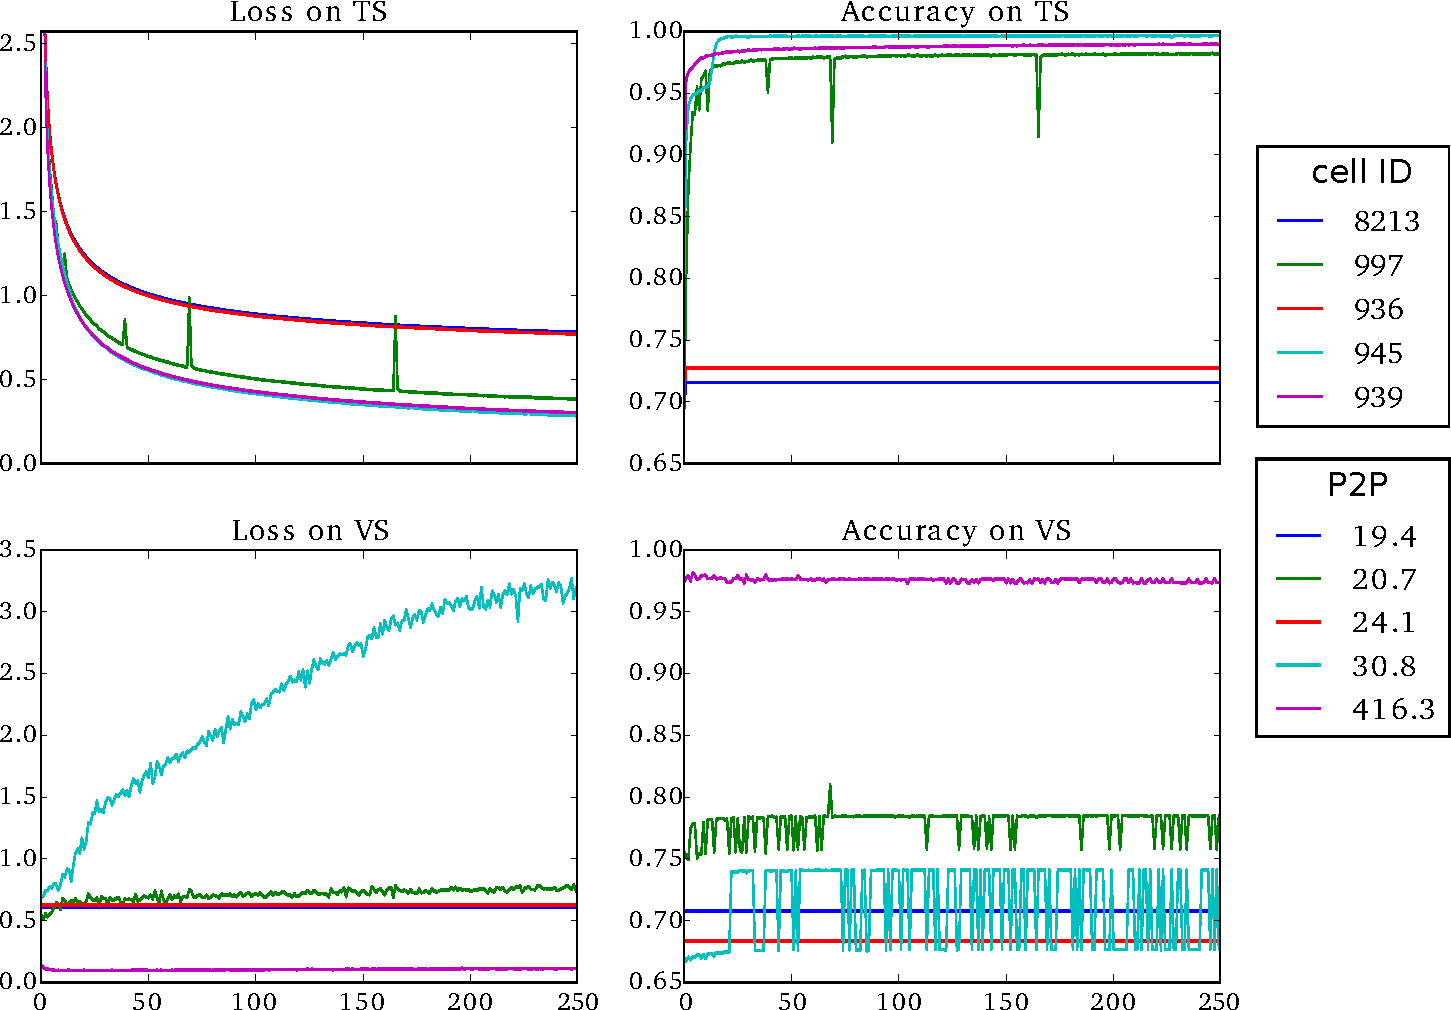
\includegraphics[width=\linewidth]{3.Chapter/study-on-different-cells-norm.pdf}
	\caption{Study on Different Recordings. Loss function and accuracies in the training set and in the validation set.The learning rate was $\eta = 0.01$, the weight decay was fixed at $\lambda = 0.001$, and the initialization method was LeCun Uniform. On the legend on the top is the Cell ID and on the legend on the bottom are the P2P amplitude (in $\mu V$).
}
\label{fig:study-cells}
\end{figure}

The values for the True Positives (TP), True Negatives (TN), False Positives (FP) and False Negatives (FN) at the end of traning were calculated as well as the values for the True Positive Rate (TPR), calculated as :
\begin{equation}
\centering
TPR = \frac{TP}{TP + FN}
\end{equation}

The results are presented in Table \ref{table:confusion-matrix}.

\begin{table}[htb]
\begin{center}
\begin{tabular}{c|cccc|cc}
cell ID & TP & TN & FP & FN & TPR & phy acc.\\ \hline
8213 & 0.00\% & 70.76\% & 0.00\% & 29.24\% & 0.00\% & -0.01\% \\
936 & 0.00\% & 68.35\% & 0.00\% & 31.65\% & 0.00\% & -1.02\% \\ 
939 & 26.85\% & 70.53\% & 0.38\% & 2.24\% & 92.31\% & 46.60\% \\ 
945 & 6.45\% & 67.66\% & 0.07\% & 25.81\% & 20.00\% & 8.38\% \\ 
997 & 2.67\% & 75.80\% & 0.18\% & 21.35\% & 11.11\% & 1.99\% \\ 
\end{tabular}
\end{center}
\caption{Values of the True Positives (TP), True Negatives (TN), False Positives (FP) and False Negatives (FN) at the end of the training, along with the value of the True Positive Rate (TPR). The accuracies achieved with phy in Chapter 2 are also presented. }
\label{table:confusion-matrix}
\end{table}

With the recordings 8213 and 936, the DNN converged to the "zero" solution since the very first epoch and was never able to be "trained out" of the local minimum it got held in. Indeed, in Table \ref{table:confusion-matrix}, the number of false negatives equals the fraction of "1" examples after upsampling (see Table \ref{table:summary-afterUS}).

The recordings 945 and 997 kept oscillating between two "states". In both cases the state with the lowest accuracy corresponds to the "zero" solution, successfully classifying all the "0" labeled examples but failing in the examples labeled as "1". In the other state, the network seems to positively classify 20.0\% and 11.11\% of the "1" examples, respectively.

Trained with the recording from the cell 939, the DNN managed to correctly classify 92.31\% of the EAPs present. 

\section{Discussion}
\label{sec:chap3-discussion}


Looking at Fig. \ref{fig:study-cells} it can be seen that with the chosen training configuration all recordings trained the DNN after only a few epochs: by the epoch 20 the accuracies in all cases reached their final value, or even getting worse afterwards, and therefore applying a stop criteria should be considered.

%%%%%%%%%%%%%%%%%%%%%%   COMPARISON WITH PHY    %%%%%%%%%%%%
Comparing with the results using phy presented in Chapter 2, this method seems to give better results: when the network didn't converge to the "zero" solution, the detection rates more than doubled, reaching a 5-fold increase on the recording 997. However, the detection rates on the recordings 945 and 997 correspond to the detection of only one spike, since the validation set in these case only had 5 and 9 different positive examples. 

It is also important to refer that the oscillations observed with the recording 945 and 997 suggest that the training used work may not be very robust: it appears that the network "jumps" easily between two local minima. Therefore it seems imperative to trained the network with more data. Another possible improvement would be increasing the probability parameter on the dropout procedure.

The recording 939 trained the network into detecting 92.31\%, which is a large value, with very few false positives and false negatives. However, in this recording the P2P amplitude was 416.3 $\mu V$, with a noise standard deviation of 10.51 $\mu V$, and should be easily detected with the conservative application of classic methods such as a threshold-based detection.
%Nonetheless, this method seems to be able to deal with situation of overlapping spikes. 
%As it was discussed in Chapter 2, probably the number of events detected by phy in this recording is underestimated and thus the improvement in this dataset may not be a big as it may seem.

In reality, the configurations and hyperparameters considered optimal were only studied with the recording 939 and may not be optimal for all datasets.

It should be noted that it is very likely that the windows labeled as "0" have many other spikes. This may actually make the training process much more difficult: since the production of any EAP relies on similar physical process, many spikes may be very similar to the spike from the juxta neuron, making the distinction, and thus the training, more difficult. For this reason, using a bigger dataset should return significantly better results, in particular, a bigger dataset with more different positive examples. The upsampling step may have forced the training to give a larger importance to each positive example but it didn't feed the network any new information about the event of interest. Possibly it could have been better to, instead of upsampling, perform downsampling or both: reduce the number of negative examples and increase the number of positive examples. In this way, more variability on the positive examples would be taken into consideration, making the network learn the useful structure of the EAPs better.

In the recording 8213 there were 202 different positive examples in the training set, more or less the same as in recording 939 which had 207. Nonetheless, the DNN was trained into the "zero" solution. At the same time this recording was the lowest in amplitude, with a $19.4 \mu V$ P2P amplitude, and the one with the highest noise standard deviation of $12.95 \mu V$, therefore most of the example are probably "drowned" in the noise, preventing the DNN to see the signal of interest. This suggests that there may be a threshold SNR below which this method cannot be applied, perhaps regardless of how many spikes there are in the training set.

It is important to keep in mind the question we're training the network to answer: whether or not, in a certain time window, there was a spike from this particular cell, and not a spike from any cell. Indeed, each network was trained with only one dataset individually. It would be interesting to train a DNN with different datasets recorded with the same probe. In this situation the question would be different: in this time window is a there a spike from this set of targeted cells? This would not only increase the number of examples (in particular positive examples), but also make this procedure more generalizable and applicable in more situations when enough different datasets have been used. However, this would affect the training: it may make it easier if the datasets are similar, or it may make it harder if there is a big difference in  EAPs from the considered juxta neurons. 

It is never too much noting that this new dataset would have to shuffled if the training algorithm doesn't do it for us, for instance if we train the network in chunks of data due to memory contraints. Otherwise, on the first epochs of training the DNN would "crystalize" on detecting that particular first EAP and may be harder to train it away from that configuration to learn the new EAPs. 
Another way to achieve this would be producing a hybrid dataset where many ground truth datasets are brought together, for examples as an average or hand-crafted, to produce one simulated recording with larger variability on the positive examples without increasing the size of the dataset, and therefore improving the unbalance in the dataset.

As mentioned above, due to memory the time windows were time shifted from the previous by 5 samples. Windows whose central sample were closest to each time juxta time where labeled as positives. Therefore if sequential time windows were presented, the DNN would probably yield 5  positive predictions per juxta spike.
\cleardoublepage
